\documentclass{article}
\usepackage{hyperref}
\usepackage{graphicx}
\graphicspath{ {figures/} }

\begin{document}

\newcommand{\link}[2]{\textbf{\href{#1}{#2}}}

\title{Wargame: Red Dragon Internal Mechanics Manual}
\date{\today}
\author{Resident Mario}
\maketitle

\newpage
\tableofcontents
\newpage

\section{Introduction}

This document lays out the structure and internal mechanics of the units in RTS video game Wargame: Red Dragon (and thereof, of the entire Wargame series). Over the course of its release the series has garnered a sizable modding community, one which has done much great work tinkering with the game and exploring the boundaries it lays out. Much credit goes in particular to Enohka, whose \link{https://github.com/enohka/moddingSuite}{Wargame Modding Suite} makes studying and patching the game's files  easy and intuitive (or at least as easy and intuitive as modifying a game of this complexity can be).

This document was prepared and published in support of an initiative in the \link{https://github.com/ResidentMario/wargame-data}{extraction and datafication} of the 1,800+ units in Wargame: Red Dragon. In its attempt to summarize in detail all that is known about the game units' interals it has many precursors. Although there are other aspects to modding, unit creation and modification is easily the most heavily travelled and easiest aspect to modding the game, and it is the explicit focus of this text.

All numbers and counts in this guide refer to Wargame: Red Dragon circa late-2016, version 510049986.

\newpage

\section{Getting Started}

This guide is written from the perspective of the Wargame Modding Suite. If you have not done so already, download this wonderful tool and point it to the most recent version of your game (refer to documentation elsewhere for instructions on how to do that).

Wargame: Red Dragon internals are organized in terms of files of the "ndfbin" type. The most important of these is "everything.ndfbin", which contains nearly all easily modifiable attributes of the game. This file, decompiled by the Modding Suite, in turn consists of a couple hundred tables. These tables, or "modules", are linked to one another within a complex hierarchy.

The most important table, for our purposes, is TUniteAuSolDescriptor. This table is top-level object describing all of the purchasable and playable units in the game (as well as a variety of deprecated and occassional "special" ones):

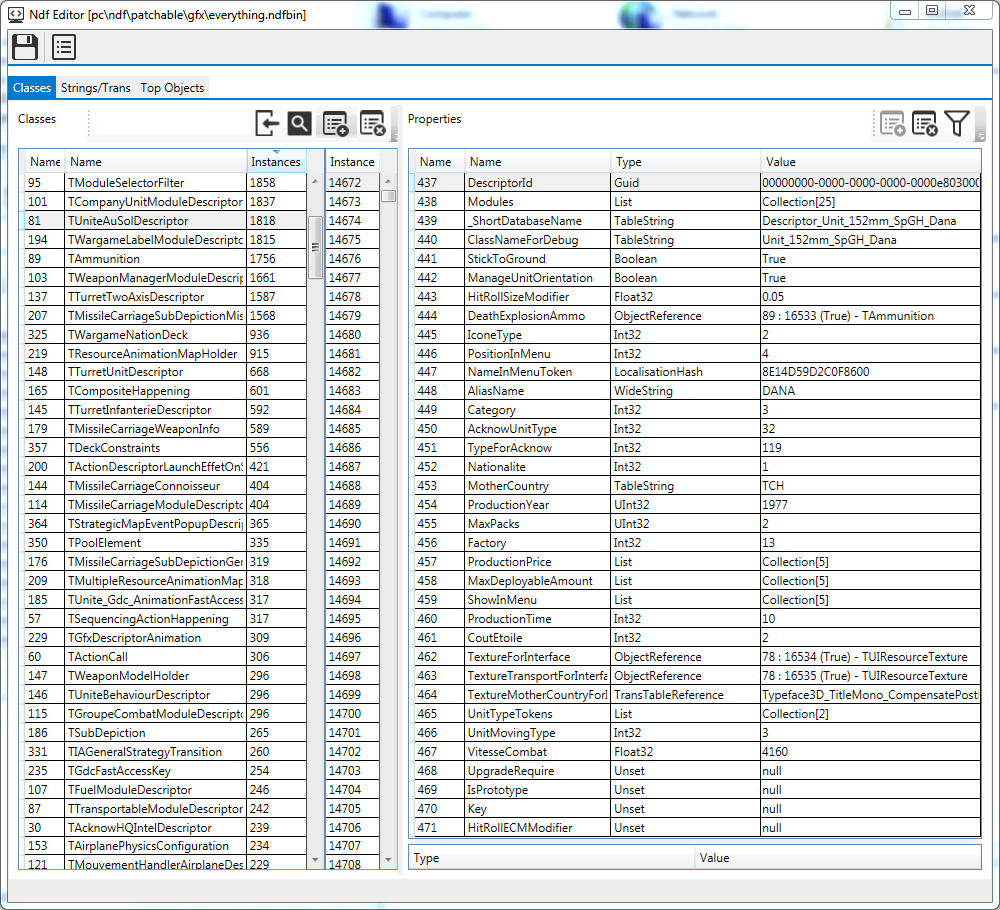
\includegraphics[width=0.8\textwidth]{screenshot_everything}


A sister table, TUniteDescriptor, describes both these units and additionally missiles, leading to a first, mildly amusing observation: missiles in the game are treated as their own units by the engine.

This table is our starting point.

Note that the first entry in this table is the 90-point Czech DANA artillery piece, which happens to, arbitrarily, have the lowest table ID in the game. This is followed by a Polish KUB-M anti-air unit, and then by a Russian Tunguska anit-air unit, as good a starting point as any other. 

\newpage

\section{TUniteAuSolDescriptor}

\subsection{DescriptorId}

This is a multi-part hex hash that is used internally by the engine. It is a unique key for the table. Don't touch it.

\subsection{\_ShortDatabaseName}

Prepended version of \_ClassNameForDebug.

\subsection{\_ClassNameForDebug}

An always-present non-localized unit name. Sometimes not entirely serious: for instance, Li Jian are given the moniker "Chinese Swords", while South Korean elite spec ops are "Black Berets". Not the name displayed in-game.

\subsection{StickToGround}

True if the unit is a helicopter, else null.

Unkown: does this have any effect?

\subsection{ManageUnitOrientation}

Null for infantry units, True otherwise.

Infantry are implemented as a special kind of vehicle in-game, and this flag likely tells the engine to treat them in some special way. But its precise effect is unknown.

See also AutoOrientation in MouvementManager.

\subsection{HitRollSizeModifier}

The effect that the size of the unit has on the chance-to-hit of other units firing at it. Larger-than-average units have a high HitRollSizeModifier, smaller-than-average ones have a low HitRollSizeModifier. This statistic is one of many calculations that factors into chance-to-hit.

The "Size" statistic in the armory screen is a direct translation of this variable. May be set to any float, but the values used in-game are:

\begin{center}
    \begin{tabular}{ | l | l | l | l | l |}
    \hline
	Value & Armory & Applies To & Example & Instances \\ \hline
	-0.2  &  Very Small & Scout helos & AH6C Little Bird  & 37\\
	-0.15 & Very Small & Infantry & Morskaya Pehota & 296 \\
	-0.1 & Very Small & Light helos & MI2URPG & 20 \\
	-0.05 & Small & Light vehicles & Scorpion Light Tank & 20\\
	null & Medium & Most things & BMP-1K & 958 \\
	0.05 & Big & Tanks, Heavy AA & M11P Abrams & 237\\
	0.1 & Very Big & Large helos & Mi-26 & 9\\	
    \hline
    \end{tabular}
\end{center}

\subsection{DeathExplosionAmmo}

A reference to a TAmmunition module which explodes in-place when this unit dies. This is a clever secondary use of TAmmunition, which is covered elsewhere in this guide.

At present time, units explode with one of just 11 animations. This includes null (e.g. no animation) which probably in error applies only to the Polish Star 266 supply truck.

\subsection{IconeType}

Speculatively, appears to control the light blue overlay that appears when using a unit to target another unit. Options are 1 (default), 2 (artillery and anti-ship missiles), and 3 (anti-air).

\subsection{PositionInMenu}

Don't know.

\subsection{NameInMenuToken}

This localization hash controls the display name of the unit in the menu. So for example if you were to want to change the name of this unit to that of another unit, inject the designated unit's token into the source unit's token.

\subsection{AliasName}

A better-formed name for the unit. Does nothing in-game. Not editable. Units which have localized names do not have an AliasName, e.g. this entry is simply null.

\subsection{Category}

Unknown.

\subsection{AcknowUnitTpye}

Unknown.

\subsection{TypeForAcknow}

Unknown.

\subsection{Nationalite}

NATO units are null, PACT units are 1.

\subsection{MotherCountry}

An abbreviation for the country of origin of this unit. Currently one of 'URSS', 'US', 'POL', 'RDA', 'CHI', 'NK', 'TCH', 'ISR', 'UK', 'FR', 'RFA', 'ROK', 'HOL', 'ANZ', 'CAN', 'SWE', 'JAP', 'DAN', 'NOR'. Note that these are French acronyms, hence why URSS is "backwards".

\subsection{ProductionYear}

The year that the unit was produced. This is the only unit of text contained in everything.ndfbin which is reproduced faithfully in-game in the armory.

\subsection{MaxPacks}

The number of cards of this infantry which are available for deck-building. Ranges from 1 (542 instances) or 2 (995 instances, the most common) up to 9 (16 instances, for certain transports).

\subsection{Factory}

Armory tab. Values are:

\begin{center}
    \begin{tabular}{ | l | l | l |}
    \hline
	Value & Tab & Count\\ \hline
	3 & Logistics & 177\\
	6 & Infantry & 233\\
	7 & Planes & 214\\
	8 & Vehicles & 335\\
	9 & Tanks & 196\\
	10 & Recon & 197\\
	11 & Helicopters & 142\\
	12 & Ships & 65\\
	13 & Anti-Air & 259\\
    \hline
    \end{tabular}
\end{center}

\subsection{ProductionPrice}

The in-game production price. This value isn't provided straight, but is instead embedded into a Collection of five integer elements. This means that production price may have originally been intended to be dependent on the veterancy of the unit, but this mechanic is not used in-game. Instead, the first value in this list is the actual price, and the remainder are all placeholder values of 15.

\subsection{MaxDeployableAmount}

A Collection of integers. The amount of copies of this unit deployable at each veterancy level, per card. 0 for veterancies this unit is not available at.

\subsection{ShowInMenu}

A Collection of booleans which is always set to True for true units and always set to False for missiles.

\subsection{ProductionTime}

How long it takes, between an air unit being clicked on or a land unit being places on the map, for the unit to appear where it's expected. Airplanes have a ProductionTime of null (instantaneous), most units have a ProductionTime of 10, and helicopters have a ProductionTime of 5. This value is in seconds.

\subsection{CoutEtiole}

Means "Price Star" in French. A quickly-dropped mechanic in the first iteration of the series, Wargame: European Escalation, was that unit cards for your deck, besides the basic ones, would cost an in-game currency known as "stars" to unlock. This variable used to control this cost, and continues to exist today as a holdover. Seems to always be set to 1, 2, or 3, and doesn't do anything.

\subsection{TextureForInterface}

A reference to the texture resource for this object's deck display.

\subsection{TextureTransportForInterface}

Transport units can appear in the armory screen as seperate units, but most of the time they are viewed during deck building "behind" the units they are carrying, in which case this texture reference is called up and placed. Is set to null for non-transport units.

\subsection{TextureMotherCountryForInterface}

Controls which flag gets displayed in the corner of the card display.

\subsection{UnitTypeTokens}

A list of LocalizationHash instances which control which armory-screen filters the unit falls inside of.

\subsection{UnitMovingType}

Flags the unit movement type. Values are:

\begin{center}
    \begin{tabular}{ | l | l | l |}
    \hline
	Value & Kind & Count\\ \hline
	1 & Foot & 296\\
	2 & Wheeled, Supply Truck, Land-Only & 36\\
	3 & Wheeled, Non-Supply Truck, Land-Only & 215\\
	5 & Tracked, Land-Only & 445\\
	6 & Planes, Helicopters & 448\\
	7 & Wheeled, Amphibious & 121\\
	8 & Tracked, Amphibious & 225\\
	9 & Ship & 32\\
    \hline
    \end{tabular}
\end{center}

A unit's track style controls how it moves, and this field contains some important information on this subject.

Units moving on foot (1) move at the same speed on land everywhere, can move on steep slopes, and cannot enter water. 

Wheeled units in general (2, 3, 7) move at 150 kph on roads, regardless of off-road speed (specified in MouvementManager), and move at 33\% of their off-road speed in forests. Amphibious wheeled units (7) can additionally enter water, moving at a globally-set 50\% of their off-road speed when doing so. I do not know what the difference between (2) and (3) is.

Tracked units in general (5, 8) move at 110 kph on roads, regardless of off-road speed (specified in MouvementManager), and move at 50\% of their off-road speed in forests. Amphibious tracked units (8) can additionally enter water, moving at a globally-set 50\% of their off-road speed when doing so.

\subsection{VitesseCombat}

The speed of the unit when it is in combat (e.g. whenever the unit can see enemy units). It is surprising that this is a top-level variable. The input is an unsigned int; for information on what the unit of measurement is, refer elsewhere in this guide.

\subsection{UpgradeRequired}

Contains a reference to another TUniteAuSolDescriptor. When this unit is pulled up in the armory, assuming you did all of the other categorization placements right, this unit will display after the linked unit in the horizontal list. If this is set to null, the unit will appear either on its own line or as the first unit in the horizontal list, if another unit references it itself.

\subsection{IsPrototype}

Whether or not the unit is a prototypal unit. Null if it isn't, True if it is. Affects deck-building, as prototypal units can't be used in global decks.

\subsection{Key}

Unknown. Almost always null.

\subsection{HitRollECMModifier}

The unit's ECM level. This only applies to planes and ships with higher than 0\% ECM; all other units (including planes without ECM) have this value set to null.

\subsection{Modules}

A list of submodules attached to this unit:


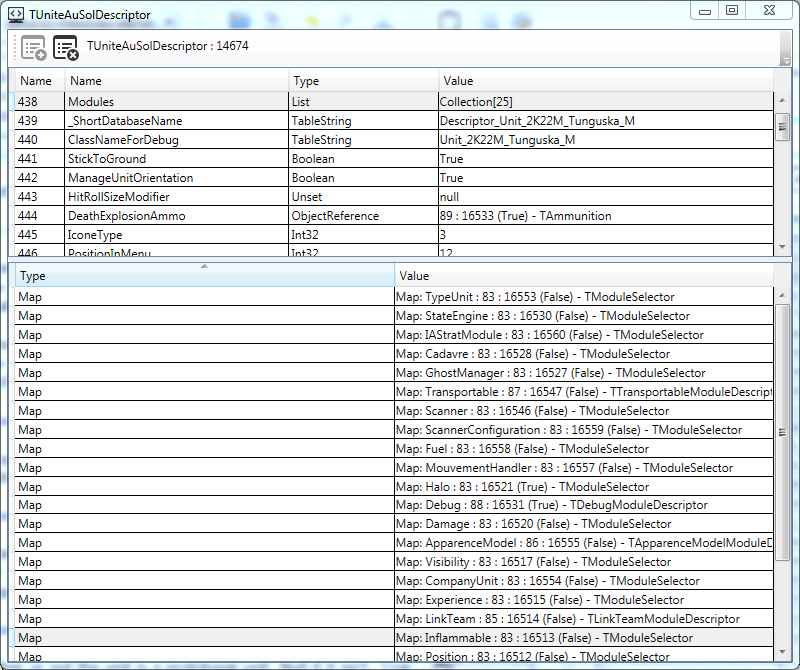
\includegraphics[width=0.8\textwidth]{screenshot_modules}

Each of these passes through a TModuleSelector to another table of some kind. We will now go through each of these in order of appearance.

\section{TTypeUnitModuleDescriptor}

\subsection{ControllerName}

Always TypeUnitController. Immutable.

\subsection{TypeUnitValue}

Unknown.

\subsection{TypeUnitHintToken}

Unknown.

\subsection{NameInMenuToken}

A copy of the top-level attribute.

\subsection{GenerateName}

Unknown. Always True.

\subsection{Filters}

Unknown. May have to do with which filters this unit falls under in the armory.

\subsection{MotherCountry}

A copy of the top-level attribute.

\subsection{UnitInfoJaugeType}

Unknown.

\subsection{Training}

Unknown. Usually, maybe always null.

\subsection{CIWS}

The CIWS statistic, as displayed in the armory, carried by a naval unit. Set to null for non-naval units and for naval units without CIWS. This is a localization hash; to set it to a particular value, use one of the following:

Exceptional = 4F233E0000000000
Very Good = 4E96452000000000
Good = 4E96450000000000
Medium = D672711906000000
Bad = CEC2000000000000
None = Set the value to null.

Changing this value does NOT change a ship's CIWS, it only changes the quality of CIWS reported on the card in-game. In other words, this only controls a text display element.

\subsection{Sailing}

The ship's sailing type. This is similarly a LocalizationHash controlling a text display, not the real value (which is in MouvementControl). We don't have an equivalency table at hand, sorry.

\section{TDebugModuleDescriptor}

There is nothing interesting here.

\section{TStateEngineModuleDescriptor}

There is nothing interesting here.

\section{TIAStratModule}

This module contains a few hard-coded numerical references which are used for internal AI orchestration.

\section{TModernWarfareCadavreModuleDescriptor}

This module is buried in the logic section of the CadavreController top-level module object. It contains a number of interesting variables, all controlling what happens when a unit dies: how long it sticks around afterwards, how quickly it fades, whether or not it exploded on death (if it does, it uses the DeathExplosionAmmo top-level object), and a bunch of flags:

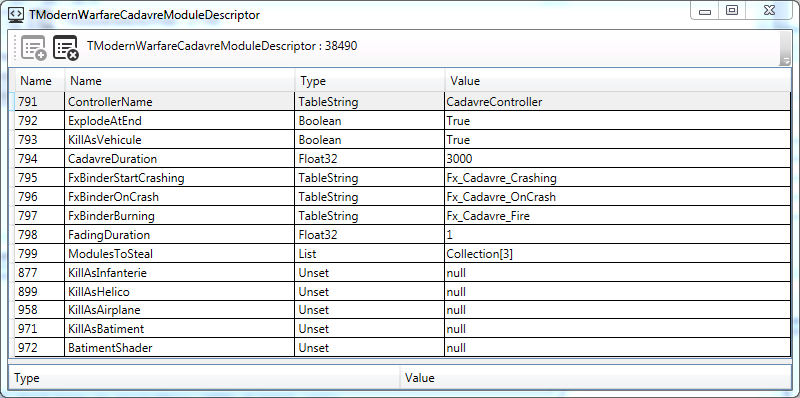
\includegraphics[width=0.8\textwidth]{screenshot_cadavre}

We will omit examining it in detail.

\section{TTurretSkeletonModuleDescriptor}

Contains a pointer to the unit's primary mesh.

\section{TMissileCarriageModuleDescriptor}

Contains pointers to art resources constituting missile carraiges (which get reused).

\section{TCommandManagerModuleDescriptor}

When this module is set up properly, the unit is treated as a command unit in-game.

\section{TGhostManagerModuleDescriptor}

Unknown.

\section{TScannerModuleDescriptor}

This module is only present if the unit has special vision privileges. It contains a TModernWarfareVisibilityRollRule as a subtable, which in turn contains TModernWarfareVisibilityRollRuleDescriptor and TModernWarfareDistanceMultiplierRollRuleDescriptor dependencies.

A relatively small number of tables of the latter two types ultimately control large swatches of unit vision ranges, so you might find that e.g. tweaking one Very Good recon unit's table's vision range up will turn up vision for ALL Very Good recon units, and other similar shenanigans.

Types of vision controlled by this module are Air, Sea, and Land.

This module only contains multipliers. Base vision values are set by the module below.

\section{TScannerConfigurationDescriptor}

This module, if present, controls the base vision values for units granted above-normal vision. All of the base values come from here, but interact with values in TScannerModuleDescriptor above. If one of these two modules is present, both are, as they are dependent on one another.

\subsection{ControllerName}

Always ScannerConfigurationController. Immutable.

\subsection{UnitType}

A reference to the domain of the unit in question itself. UnitType 1 refers to ground, UnitType 4 refers to planes, and UnitType 6 refers to ships.

\subsection{DetectionTBA}

Maximum range at which you can see an unidentified helicopter.

\subsection{PorteeVision}

Maximum range at which you can see an unidentified ground unit.

\subsection{OpticalStrength}

Optical strength against ground units, used to determine whether a unit can see enemy units in cover.

\subsection{OpticalStrengthAltitude}

Optical strength against aircraft (including helicopters).

\subsection{SpecializedOpticalStrengths}

This is a Collection of float pair mapping; each of the maps binds a UnitType and then the range at which they can be detected. UnitType 4 refers to planes, while UnitType 6 refers to ships, and UnitType 1 refers to Land. The value Optican strengths against 

\subsection{SpecializedDetections}

Maximum range at which you can see an unidentified unit. This is a Collection of float pair mapping; each of the maps binds a UnitType and then the range at which they can be detected. UnitType 4 refers to planes, while UnitType 6 refers to ships, and UnitType 1 refers to Land.

\subsection{PorteVisionTBA}

Maximum spotting range for helicopters. This attribute is only populated for helicopters, in which case it controls helicopter-to-helicopter sighting. It is otherwise null.

\subsection{OpticanStrengthAntiradar}

Maximum anti-radar spotting range. Only populated for anti-radar units; null otherwise.

\subsection{\_ShortDatabaseName}

Same as the top-level parameter, but this seems to always be null.

\section{TFuelModuleDescriptor}

\subsection{ControllerName}

Uninteresting.

\subsection{FuelCapacity}

The number of units of fuel that this unit can stockpile.

\subsection{FuelMoveDuration}

Autonomy in kilometers; the same as the statistic displayed in the Armory.

\section{TMovementHandlerLandVehicleDescriptor}

This module will only be present if the vehicle in question is, indeed, a land unit.

\subsection{ControllerName}

Uninteresting.

\subsection{Maxspeed}

The unit's max speed, in engine distance units (the meaning of which is covered elsewhere).

\subsection{UnitMovingType}

The same as that set in TUnitMouvementDescriptor.

\subsection{SpeedBonusOnRoad}

A multiplier on the unit's base speed. Always set to whatever it needs to be set to to give the unit 110kph tracked speed or 150kph wheeled speed, meaning that these are constants but must be set on the local level!

\subsection{TempsDemiTour}

The amount of time, in seconds, it takes for a unit to make a half-turn (the translation is literal). If you tell a unit to move in a direction directly opposite to its current orientation, it will do a reverse-accelerate V-turn to the side, and this variable controls how long this takes.

Presumably this value also controls how long it takes to make turns that are less than 360 degrees, but still significant. The cutoff value at which a unit starts to make a reverse turn, instead of just turning in place, is unknown.

\subsection{MaxAcceleration}

The acceleration the unit applies when it is speeding up.

\subsection{MaxDeceleration}

How hard to breaks hit. Tends to be twice MaxAcceleration for tracked and wheeled land units.

\subsection{VehicleSubType}

Unknown, often null.

\subsection{CriticalEffectModule}

A module pointer whose contents is a TCriticalEffectModuleDescriptor describing what happens when this units is hit with a critical. Unfortunately it ultimately points to hashes, not to any descriptions of the effects of the criticals themselves...

\subsection{TerrainsToIgnoreMask}

This is set to certain magic values for ship units which are allowed and not allowed to enter different water depths: 16 if it can enter all waters, 24 if it's a coaster, and 26 if it's a bluewater ship.

Otherwise null.

\section{TMouvementHandlerHelicopterDescriptor}

\subsection{ControllerName}

Uninteresting.

\subsection{Maxspeed}

The unit's max speed, in engine distance units (the meaning of which is covered elsewhere).

\subsection{MaxAcceleration}

The acceleration the unit applies when it is speeding up.

\subsection{MaxDeceleration}

How hard the breaks hit.

\subsection{UnitMovingType}

The same as that set in TUnitMouvementDescriptor. Here this will always be 6, for air.

\subsection{CyclicManoeuvrability}

Controls movement.

\subsection{GFactorLimit}

Controls movement.

\subsection{LateralSpeed}

Controls movement.

\subsection{Mass}

Controls movement.

\subsection{MaxInclination}

Controls movement.

\subsection{RotorArea}

Controls movement.

\subsection{TorqueManoeuvrability}

Controls movement.

\subsection{UpwardsSpeed}

Controls movement.

\subsection{CriticalEffectsModule}

A module pointer whose contents is a TCriticalEffectModuleDescriptor describing what happens when this units is hit with a critical. Unfortunately it ultimately points to hashes, not to any descriptions of the effects of the criticals themselves...

\subsection{TempsDemiTour}

The amount of time, in seconds, it takes for a unit to make a half-turn (the translation is literal). For helicopters this requires a dive to the left. It's uncertain whether or not this variable is still used for anything.

\section{TMouvementHandlerAirplaneDescriptor}

\subsection{Maxspeed}

Maximum speed this unit can go at. Since airplanes fly at a constant speed, this is also the only speed.

\subsection{UnitMovingType}

Always 6, for air (other values are 4 for sea and 1 for land).

\subsection{FlyingAltitude}

The height the plane usually flies at.

\subsection{MinimalAltitude}

Below which the plane will not dip. Will cause it to break off from certain attacks at certain heights.

\subsection{PhysicsConfiguration}

A reference to a TAirplanePhysicsConfiguration module, which controls the plane's various movement parameters.

\subsection{CriticalEffectsModule}

A module pointer whose contents is a TCriticalEffectModuleDescriptor describing what happens when this units is hit with a critical. Unfortunately it ultimately points to hashes, not to any descriptions of the effects of the criticals themselves...

\subsection{GunMuzzleSpeed}

Unknown. Always 300000.

\subsection{LandingGearOutPhysicalPropertyName}

Unknown. Always "InShowRoom".

\subsection{LandingGearSubDescriptionName}

Unknown. Always "Landing Gear".

\subsection{FrontLandingGearMeshNodeName}

Unknown. Always "Train\_Avant".

\subsection{BackLandingGearMeshNodeName}

Unknown. Always "Train\_Arriere".

\section{THaloModuleDescriptor}

Does a bunch of things which control the circle that gets drawn when a unit is selected.

\section{TWeaponManagerDescriptor}

\section{TModernWarfareDamageModuleDescriptor}

\section{TAppearanceModelDescriptor}

Controller for things related to the unit's appearance.

\section{TVisibilityModuleDescriptor}

\subsection{ControllerName}

Uninteresting.

\subsection{UnitStealthBonus}

A multiplier applied to the unit's visibility, and the only interesting contents of this module. The multipliers are:

\begin{center}
    \begin{tabular}{ | l | l | l | l |}
    \hline
	Value & Stealth & Examples & Counts\\ \hline
	0.1 & Bad & Hatsuyiki & 1\\
	0.3 & Bad & Luda & 1\\
	0.4 & Bad & Oliver Hazard Perry & 1\\
	0.5 & Bad & Jianghu III & 3\\
	0.6 & Bad & Nanushka III & 4\\
	0.7 & Bad & Donghae & 5\\
	0.8 & Bad & Chamsuri & 4\\
	0.9 & Bad & Shmel & 2\\
	1 & Poor & AMX-30B & 1349\\
	1.2 & Medium & Komar & 1\\
	1.25 & Poor (!) & MiG-29S & 1\\
	1.5 & Medium & VLB Minstral Recon & 139\\
	1.75 & Good & PAH-2 Tiger & 4\\
	2 & Good & US Marines & 200\\
	2.5 & Very Good & Spetsnaz GRU & 91\\
	3 & Exceptional & Spetsnaz VMF, Nighthawk & 7\\
    \hline
    \end{tabular}
\end{center}

\subsection{\_ShortDatabaseName}

The same as that set in the top-level object, but seemingly always null.

\section{TCompanyUnitDescriptor}

Companies are what the game terms sets of units ranging in size from 1 (lone) to 4 (max size; helicopters can only be grouped in 2s and planes and boats in 1s). This module contains a bunch of elements which define the logic of giving orders to a company of units, as well as the number limiting how many of the unit stack.

\end{document}